\addcontentsline{toc}{subsubsection}{Graph Transformation: Modulus}
\vbtitle{\textbf{Graph Transformation: Modulus}}

\begin{enumerate}
    \item $|x|+|y|=1$
        \begin{multicols}{2}
            \begin{align*}
                \intertext{\textbf{Step 1:}}
                \intertext{Start with simple standard equations:}
                \intertext{In this case we have:}
                x + y &= 1\\[10mm]
            \end{align*}
            \begin{center}
            \begin{tikzpicture}
            [scale=1.25]
                \tzaxes(-2, -2)(2,2){$x$}{$y$}
                \tzticksx*(-2pt:2pt){-1, 1} 
                \tzticksy*(-2pt:2pt){-1, 1}
                \tzfn{1-\x}[-1:2]
            \end{tikzpicture}
            \end{center}
        \end{multicols}
        \begin{multicols}{2}
            \begin{align*}
                \intertext{\textbf{Step 2:}}
                \intertext{Apply modulus transformation to $x$:}
                \intertext{Applying modulus to $x$ means that the graph will be reflected about the y-axis.}
                \intertext{Try to understand why it gets reflected, $|-2|=|2|=2$, for positive input modulus does nothing, so plotted for $x \geq 0$ and we know it will give the same output for $x < 0$. Graphically this can be achieved by reflecting the graph($x \geq 0$) about the y-axis.}
                |x| + y &= 1\\[1mm]
            \end{align*}
            \begin{center}
                \begin{tikzpicture}
                    [scale=1.25]
                        \tzaxes(-2, -2)(2,2){$x$}{$y$}
                        \tzticksx*(-2pt:2pt){-1, 1} 
                        \tzticksy*(-2pt:2pt){-1, 1}
                        \tzfn[dashed]{1-\x}[-1:0]
                        \tzfn{1-abs(\x)}[-2:2]
                    \end{tikzpicture}
            \end{center}
        \end{multicols}
        \begin{multicols}{2}
            \begin{align*}
                \intertext{\textbf{Step 3:}}
                \intertext{Apply modulus transformation to $y$:}
                \intertext{Applying modulus to $y$ means that the graph will be reflected about the x-axis.}
                \intertext{Again, same idea but this time for $y$.}
                |x| + |y| &= 1\\[1mm]
            \end{align*}
            \begin{center}
                \begin{tikzpicture}
                    [scale=1.25]
                        \tzaxes(-2, -2)(2,2){$x$}{$y$}
                        \tzticksx*(-2pt:2pt){-1, 1} 
                        \tzticksy*(-2pt:2pt){-1, 1}
                        \tzfn[dashed]{1-abs(\x)}[-2:-1]
                        \tzfn[dashed]{1-abs(\x)}[1:2]
                        \tzfn{1-abs(\x)}[-1:1]
                        \tzfn{abs(\x)-1}[-1:1]
                    \end{tikzpicture}
            \end{center}
        \end{multicols}

    \item $|x|-|y|=1$
        \begin{multicols}{2}
            \begin{align*}
                \intertext{\textbf{Step 1:}}
                \intertext{Start with simple standard equations:}
                \intertext{In this case we have:}
                x - y &= 1\\[10mm]
            \end{align*}
            \begin{center}
            \begin{tikzpicture}
            [scale=1.25]
                \tzaxes(-2, -2)(2,2){$x$}{$y$}
                \tzticksx*(-2pt:2pt){-1, 1} 
                \tzticksy*(-2pt:2pt){-1, 1}
                \tzfn{\x-1}[-1:2]
            \end{tikzpicture}
            \end{center}
        \end{multicols}
        \begin{multicols}{2}
            \begin{align*}
                \intertext{\textbf{Step 2:}}
                \intertext{Apply modulus transformation to $x$:}
                \intertext{Applying modulus to $x$ means that the graph will be reflected about the y-axis.}
                |x| - y &= 1\\[1mm]
            \end{align*}
            \begin{center}
                \begin{tikzpicture}
                    [scale=1.25]
                        \tzaxes(-2, -2)(2,2){$x$}{$y$}
                        \tzticksx*(-2pt:2pt){-1, 1} 
                        \tzticksy*(-2pt:2pt){-1, 1}
                        \tzfn[dashed]{\x-1}[-1:0]
                        \tzfn{abs(\x)-1}[-2:2]
                    \end{tikzpicture}
            \end{center}
        \end{multicols}
        \begin{multicols}{2}
            \begin{align*}
                \intertext{\textbf{Step 3:}}
                \intertext{Apply modulus transformation to $y$:}
                \intertext{Applying modulus to $y$ means that the graph will be reflected about the x-axis.}
                |x| - |y| &= 1\\[1mm]
            \end{align*}
            \begin{center}
                \begin{tikzpicture}
                    [scale=1.5]
                    \tzaxes(-2, -2)(2,2){$x$}{$y$}
                    \tzticksx*(-2pt:2pt){-1, 1} 
                    \tzticksy*(-2pt:2pt){-1, 1}
                    \tzfn[dashed]{abs(\x)-1}[-1:1]
                    
                    \tzfn{abs(\x)-1}[-2:-1]
                    \tzfn{abs(\x)-1}[1:2]
                    
                    \tzfn{1-abs(\x)}[-2:-1]
                    \tzfn{1-abs(\x)}[1:2]
                \end{tikzpicture}
            \end{center}
        \end{multicols}
    
    \item $y=|x|$
        \begin{multicols}{2}
            \begin{align*}
                \intertext{\textbf{Step 1:}}
                \intertext{Start with simple standard equations:}
                \intertext{In this case we have:}
                y &= x\\[10mm]
            \end{align*}
            \begin{center}
            \begin{tikzpicture}
            [scale=1.25]
                \tzaxes(-2, -2)(2,2){$x$}{$y$}
                \tzticksx*(-2pt:2pt){-1, 1} 
                \tzticksy*(-2pt:2pt){-1, 1}
                \tzfn{\x}[-2:2]
            \end{tikzpicture}
            \end{center}
        \end{multicols}
        \begin{multicols}{2}
            \begin{align*}
                \intertext{\textbf{Step 2:}}
                \intertext{Apply modulus transformation to $x$:}
                \intertext{Applying modulus to $x$ means that the graph will be reflected about the y-axis.}
                |x| &= y\\[1mm]
            \end{align*}
            \begin{center}
                \begin{tikzpicture}
                    [scale=1.25]
                        \tzaxes(-2, -2)(2,2){$x$}{$y$}
                        \tzticksx*(-2pt:2pt){-1, 1} 
                        \tzticksy*(-2pt:2pt){-1, 1}
                        \tzfn[dashed]{\x}[-2:0]
                        \tzfn{-\x}[-2:0]
                        \tzfn{\x}[0:2]
                    \end{tikzpicture}
            \end{center}
        \end{multicols}
\pagebreak
    \item $|y|= e^{-|x|}$
        \begin{multicols}{2}
            \begin{align*}
                \intertext{\textbf{Step 1:}}
                \intertext{Start with simple standard equations:}
                \intertext{In this case we have:}
                y &= e^{-x}\\[10mm]
            \end{align*}
            \begin{center}
            \begin{tikzpicture}
            [scale=1.25]
                \tzaxes(-2, -2)(2,2){$x$}{$y$}
                \tzticksx*(-2pt:2pt){-1, 1} 
                \tzticksy*(-2pt:2pt){-1, 1}
                \tzfn{exp(-\x)}[-1:2]
            \end{tikzpicture}
            \end{center}
        \end{multicols}
        \begin{multicols}{2}
            \begin{align*}
                \intertext{\textbf{Step 2:}}
                \intertext{Apply modulus transformation to $x$:}
                \intertext{Applying modulus to $x$ means that the graph will be reflected about the y-axis.}
                e^{-|x|} &= y\\[10mm]
            \end{align*}
            \begin{center}
                \begin{tikzpicture}
                    [scale=1.25]
                        \tzaxes(-2, -2)(2,2){$x$}{$y$}
                        \tzticksx*(-2pt:2pt){-1, 1} 
                        \tzticksy*(-2pt:2pt){-1, 1}
                        \tzfn[dashed]{exp(-\x)}[-1:0]
                        \tzfn{exp(\x)}[-2:0]
                        \tzfn{exp(-\x)}[0:2]
                    \end{tikzpicture}
            \end{center}
        \end{multicols}
        \begin{multicols}{2}
            \begin{align*}
                \intertext{\textbf{Step 3:}}
                \intertext{Apply modulus transformation to $y$:}
                \intertext{Applying modulus to $y$ means that the graph will be reflected about the x-axis.}
                |y| &= e^{-|x|}\\[10mm]
            \end{align*}
            \begin{center}
                \begin{tikzpicture}
                    [scale=1.25]
                        \tzaxes(-2, -2)(2,2){$x$}{$y$}
                        \tzticksx*(-2pt:2pt){-1, 1} 
                        \tzticksy*(-2pt:2pt){-1, 1}
                        \tzfn[dashed]{exp(-\x)}[-1:0]
                        \tzfn{exp(\x)}[-2:0]
                        \tzfn{exp(-\x)}[0:2]
                        \tzfn{-exp(-\x)}[0:2]
                        \tzfn{-exp(\x)}[-2:0]
                    \end{tikzpicture}
            \end{center}
        \end{multicols}
    
\end{enumerate}


